\documentclass[tikz,border=10pt,12pt,x11names]{standalone}
\usepackage{verbatim}
%%%>
\usetikzlibrary{calc,arrows}
\usepackage{tikz}
\usepackage[]{circuitikz} % TiKZ Library for US Logic Circuits.
\usetikzlibrary{circuits.logic.US} % TiKZ Library for US Logic Circuits.
\usepackage{amsmath}

\usepackage{tikz}
\usetikzlibrary{circuits.logic.US} % TiKZ Library for US Logic Circuits.
\begin{document}
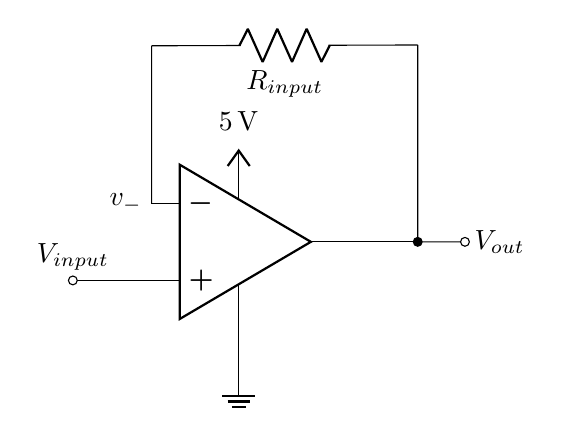
\begin{tikzpicture}[scale=2]


\draw (0,0) node[op amp] (opamp) {}
%(opamp.+) node[left] {$v_+$}
(opamp.-) node[left] {$v_-$}
(opamp.up) --++(0,0.1) node[vcc]{5\,\textnormal{V}}
(opamp.down) --++(0,-0.5) node[ground]{};

\draw (opamp.out) to[short] ([xshift=0.5cm]opamp.out) node[anchor=south east]{};

\draw ([xshift=0.5cm]opamp.out) to[short] ([xshift=0.5cm,yshift=1.25cm]opamp.out)

([xshift=0.5cm]opamp.out) to[short,*-o ] ([xshift=0.8cm]opamp.out) node[anchor=west]{$V_{out}$}


([xshift=0.5cm,yshift=1.25cm]opamp.out) to[R=$R_{input}$] ([yshift=1cm]opamp.-)

([yshift=1cm]opamp.-) to[short](opamp.-); 

\draw (opamp.+) to[short,-o] ([xshift=-0.5cm]opamp.+) node[anchor=south]{$V_{input}$}

;




\end{tikzpicture}
\end{document}